\chapter{Synchronization Plugins}
Synchronization Plugins are modules which provides access to a certain device,
application or protocol. All of those plugins provide independent of the
synchronized content/format or connection type, the same functions:
\begin{itemize}
\item initialize. This function parse the plugin configuration and initializes
the plugin. If the plugin acts as server, it also initializes this one and 
listen for incoming connections.
\item finalize. This function releases all gained memory by the plugin and stops
the listening server if present. 
\item discover. This function is intended to get called initially to gain
information about the target application, device or system. In detail it detects
all supported formats and individual capabilities of this format, if possible.
And basic information about the target application/device like version, vendor,
product, etc. ...
%\item usable. This function is intended to check if the target
%application/device is usable.
\end{itemize}

\begin{figure}
 \centering
 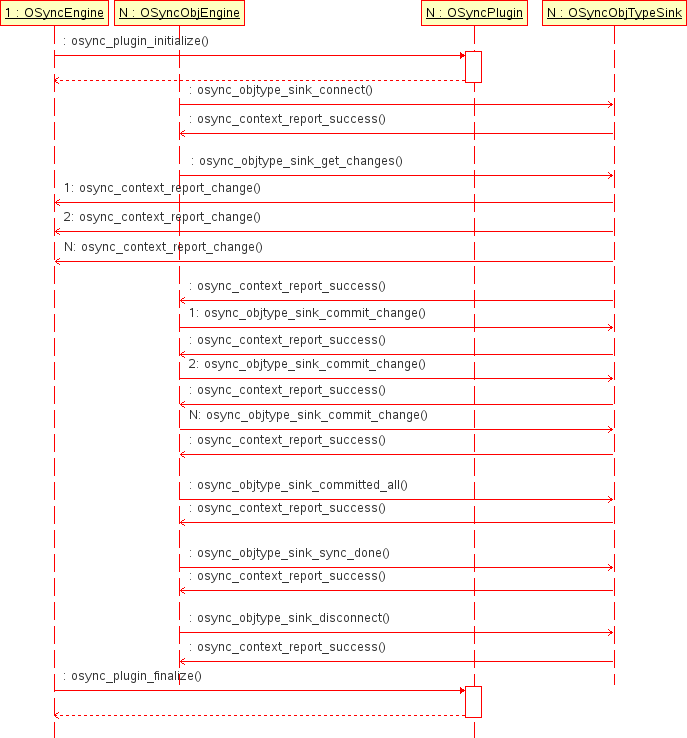
\includegraphics[bb=0 0 661 960, scale=0.60]{simple-sync-sequence}
 % simple-sync-sequence.png: 661x960 pixel, 72dpi, 23.32x33.87 cm, bb=0 0 661 960
 \caption{Plugin Synchronization Sequence}
 \label{fig:SimpleSyncSequence}
\end{figure}

Those function are called "Generic Functions" and MUST be implemented by 
plugin.

\section{Plugin module functions}
The plugin module functions are called once synchronously when the module
is loaded.
\subsection{get\_sync\_info}
This is the entry point for the plugin.  Once the plugin is loaded
\verb|get_sync_info| is called to determine the connectors provided by the
plugin. A single plugin may provide module may provide several connectors.  For
example the syncml plugin provides syncml-obex, syncml-http-client and
syncml-http-server connectors.

In this function a plugin must create an OSyncPlugin for each of the connectors
it provides.  The initialize, discover and finalize functions for each provided
conector must be set using the coressponding \verb|osync_plugin_set|
function. Each OSyncPlugin is added to the passed plugin environment using
\verb|osync_plugin_env_register_plugin|.

Return TRUE on success.  If an error occurs set OSyncError and return FALSE.
\section{Plugin specific functions}
These functions are called for a particular plugin that was registered in
\verb|get_sync_info|.
\subsection{Initialize}
The next call to the plugin will be to initialize a particular connector that
was registered in get\_sync\_info.  At this point the engine will have read the
plugin config which can be accessed using \verb|osync_plugin_info_get_config|

During this function the plugin should set itself up and register functions for each
objtype.

The passed OSyncPluginInfo contains a list of OSyncObjTypeSink.  Each of these
represents an objtype (e.g. contact, event) that the engine is capable of
syncing.  For each of these the plugin must:

Register Sink functions using \verb|osync_objtype_sink_set_functions|

If a MainSink is needed (e.g. to connect to an interface that is shared between
several objtype sinks) it can be created and registered using:
\verb|osync_objtype_main_sink_new| \verb|osync_plugin_info_set_main_sink|

The function should return it's data cast to (void *) on success.  On failure
return NULL and set OSyncError to a user friendly explaination of the failure
cause.
\subsection{Discover}
In this function the plugin reports which objtype sinks are available, sets
version information and if requiring dynamically generated capabilities reports
them here.  Initialize will already have been called.

If an objtype can be syncronized then it should be set available using
\verb|osync_objtype_sink_set_available|.  Again the OSyncPluginInfo contains a
list of objtypes known to the engine.

There are two ways to describe the capabilities of a plugin: Dynamic and Static.
Not defining any capabilties WILL lead to data loss unless your plugin supports
all possible attributes.
\subsubsection{Static Capabilties}
Static capabilities are described in xml files shipped with a plugin.  A
descriptions.xml file links OSyncVersion properties to a particular capabilites
xml file. If no capabilities are set by the plugin in discover the engine will
use the version info to find the best matching capbilities.  If several
capabilities files match then the one with the ?highest/lowest? capability is
used.

\begin{verbatim}
Use the osync_verion_set functions as required.

	OSyncVersion *version = osync_version_new(error);
	osync_version_set_plugin(version, "pluginname");
	osync_version_set_modelversion(version, "version");
	osync_version_set_firmwareversion(version, "firmwareversion");
	osync_version_set_softwareversion(version, "softwareversion");
	osync_version_set_hardwareversion(version, "hardwareversion");
	osync_plugin_info_set_version(info, version);
\end{verbatim}

\subsubsection{Dynamic capabilities generation}
If the capabilities of a peer can only be known by querying it or can not be set using the
static capabilities method. The plugin must generate the capabilities.

Create new capabilities using:
\verb|osync_capabilities_new and osync_capability_new|
Add the capabilities to the plugin info using:
\verb|osync_plugin_info_set_capabilities|
\subsection{Finalize}
Clean up and free any allocated memory
%\subsection{Usable}
\section{Sink Functions}
All "Sink Functions" are called asynchronously, and must reply with OSyncContext functions.
 It's very important that the ">Sink Functions"< reply to the
request by the OpenSync Framework with the OSyncContext functions. Even on
error condition the Sink Function have to reply with a special OSyncContext
error function. Otherwise the OpenSync Framework will wait until the timeout for this
function call is reached before failing the function.

The Main Sink, which has no object type doesn't have any required Sink 
Functions. For Object Type Sinks the implementation of some Sink 
Functions required:

\begin{center}
% use packages: array
\begin{tabular}{ll}
\textbf{Function} & \textbf{Implementation} \\ 
Connect & Optional \\
Connect Done & Optional \\
Get Changes & Required \\ 
Commit & Required \\ 
Committed All & Optional (only available in combination with Commit)\\ 
Synchronization Done & Optional \\ 
Disconnect & Optional
\end{tabular}
\end{center}

The sink for which the sink function has been called may be found using
\verb|osync_plugin_info_get_sink|

\subsection{Connect}
The Connect function is available for all Object Type Sinks and could be used to
establish Object Type specific connection. If the connection establishment is an
Object Type neutral task (e.g. Bluetooth, USB, ...) and needs to be done only
once, only the Main Sink should be given a connect function. This avoids
problems with shared access to an interface, since a connect function would
otherwise be called for each Object Type for the same interface.

It is usual at this stage to compare the stored anchor with that from the peer
using \verb|osync_sink_state_equal|.  If the anchor has changed then the need for
a slow sync should be set using \verb|osync_objtype_sink_set_slowsync|

This function MUST only establish a connection to the device or resource. After
the connection has been successfully established successful the plugin MUST
reply with \verb|osync_context_reply_success()|. On error the plugin replies
with a human-readable (aka. userfriendly) error message using
\verb|osync_context_reply_error()|.
\subsection{Connect Done}
Called after all peers have connected.  At this point the slow sync status of
all peers is known.  If your plugin must connect differently depending on the
group slow sync status then you may perform that connection here.
\subsection{Get Changes}
The Get Changes function gets called by the OpenSync Framework to request changes
since last synchronization or all entries of the Object Type specific resource.
The later case MUST be performed when a Slow Sync got requested by the OpenSync
Synchronization framework. The Slow Sync status of this Sink MUST be
checked with \verb|osync_objtype_sink_get_slowsync()|. On a Slow Sync the 
Changetype (for all changes) is \verb|OSYNC_CHANGE_TYPE_ADDED|. On a regular 
(fast sync) synchronization it's up to the Get Changes function to determine 
the Changetype. Every change has to be reported with 
\verb|osync_context_report_change()|. On error the Sink Function must
reply with \verb|osync_context_report_error()| and stop/leave this 
function ASAP. If the protocol, application or device isn't able to report 
changed entries since last sync, the OpenSync Helper Hashtable should be used 
to determine the Changetype of the entry.
\subsection{Commit}
This function get called with a single OSyncChange object, which MUST be
committed to the application or device. If the commit failed the context MUST be
replied with \verb|osync_context_report_error()|. On success the context get
replied with \verb|osync_context_success()|. If Hashtable is already involved in
the Get Changes functions, then the Commit function should update the Hashtable
for the entries which get committed.
\subsection{Committed All}
This function is called after all entries have committed, even if error appeared
while committing.
\subsection{Synchronization Done}
This function is called only after a successful synchronization.  When using a
Hashtable \verb|osync_hashtable_save()| should be called to store the Hashtable
to disk.
\subsection{Disconnect}
This function MUST only handle the disconnect of the sink. Don't do further
cleanup here, the finalize function is intended for releasing memory and
cleanup. The disconnect function ???might be called even if the connect
function failed.
\section{Properties}
Each Synchronization Plugin has properties which get set within the
\verb|get_sync_info()| function. The properties are:

\begin{itemize}
\item Name, short name of the plugin should be less then 15 characters. This
name isn't visible to the user, at least not for rich OpenSync Frontends.
\item Longname, is the name of the plugin which is visible to the user in
rich OpenSync frontends. Should not be longer then 50 characters.
\item Description, about the Plugin visible to the end user in OpenSync
Frontends, and should additionally help to choose the right plugin.
\item Configuration Type, defines if the plugins needs any configuration or if
the configuration is optional or simply not needed.
\item Process Type, defines how the plugin get started: threaded, forked or by 
an external process.
\item Timeouts, for initialization, finalization and timeout can be configured
for the plugin needs. 
\end{itemize}

\subsection{Name}
The name of the plugin get defined like all plugin properties in
\verb|get_sync_info()| function with calling \verb|osync_plugin_set_name()|.
This name got used mostly for internal configuration and isn't visible to the 
user (at least not for rich OpenSync Frontend user). The name should be less
then 15 characters and should one word (no spaces). Example: ">palm-sync"<
\subsection{Longname}
The Longname of the plugin is the only name visible for  regular user to choose 
the correct plugin from a list of available plugins. Use the description field
to describe the plugin in more detail. Don't include the term ">Plugin"> in the
Longname. Example: ">Palm Device"<
\subsection{Description}
The description should additionaltly help the user to choose the correct plugin
if there are several plugins with similar names. Bad example: ">Plugin to sync 
your pda. Version 0.23. http://foo.edu/hacking/opensync"<. The term ">Plugin"< 
might confuse regular user, avoid it. If your plugin supports several different
devices don't list all known to work models, this might confuses people as well.
Again, don't list models! If your plugin is based on a synchronization 
implementation mention the name of protocol. No version numbers, no URLs and 
most user won't care about the authors name or E-Mail address.
\subsection{Plugin Timeouts}
The default plugin timeout should basically fit the need for all plugins. If
your plugin is known to be very slow you can change the timeout for this plugin
with following functions:
\begin{itemize}
\item \verb|osync_plugin_set_initliaze_timeout()|
\item \verb|osync_plugin_set_finalize_timeout()|
\item \verb|osync_plugin_set_discover_timeout()|
%\item \verb|osync_plugin_set_useable_timeout()|
\end{itemize}
The timeout unit is in seconds. It's possible to overwrite custom plugin timeout
with setting individual timeouts in the member configuration (syncmember.conf).
\subsection{Configuration Types}
If the plugin doesn't need any configuration by the user the plugin should the
configuration type to \verb|OSYNC_PLUGIN_NO_CONFIGURATION| with the
\verb|osync_plugin_set_config_type()| function. If the plugin don't need by
default a configuration but could be is additionally configurable the
configuration type should be set to \verb|OSYNC_PLUGIN_OPTIONAL_CONFIGURATION|. 
If the plugin can't perform without any configuration the type should be set
to\\ \verb|OSYNC_PLUGIN_NEEDS_CONFIGURATION| (set by default).
\subsection{Process Types}
The Process Type declares how a plugin get started. By default the plugin get
started by the OpenSync Framework within a thread (
\verb|OSYNC_START_TYPE_THREAD|). If the Plugin is known to conflict with the 
process mainloop of the OpenSync Framework, it's possible to run the plugin in 
a separated process by forking it. The forking is done by the OpenSync
Framework when the start type got set to \verb|OSYNC_START_TYPE_PROCESS|. If the
plugin has to access a not public interface to get access to the data resources
of an application it's possible to integrate the plugin within this application.
So the plugin is running all the time this application is running and can
communicate with the OpenSync Framework when the Process Type got set to 
\verb|OSYNC_START_TYPE_EXTERNAL|. The Process Type can be changed with the 
\verb|osync_plugin_set_start_type()| function. 
\section{Configuration}
